\lstdefinelanguage[ECMAScript2015]{JavaScript}[]{JavaScript}{
  morekeywords=[1]{await, async, case, catch, class, const, default, do,
    enum, export, extends, finally, from, implements, import, instanceof,
    let, static, super, switch, throw, try},
  morestring=[b]` % Interpolation strings.
}
\lstalias[]{ES6}[ECMAScript2015]{JavaScript}


\chapter{Implementation}
% What did you do to implement this idea, and what technical achievements did you make?
% You can't talk about everything. Cover the high level first, then cover important, relevant or impressive details.

This chapter will cover the implementation details of the project, including the technologies used to develop the system, the unique and/or novel technical features of the app, and the deployment of the project onto a live website.

\section{Chosen Technologies}

\subsection{Web Framework}
The project was designed to be made as a web app from the very beginning. There are several advantages and drawbacks but ultimately this was the preferred platform to develop the project on. A web app would be the most accessible way for users to quickly access the project as no installation is required. Additionally, the project would be inherently cross-platform and viewable on a large variety of devices, further increasing the accessibility and ease of use, which was a priority.

Naturally, developing a complex application using web technologies had its drawbacks such as performance concerns. From prior experience, web apps have often required a focus on optimisation and a careful balance between practicality and seamlessness. Since there would be many audio assets which the end user would be required to download, it was important to take into account users with slower internet connections when designing the app. Furthermore, due to the many possible aspect ratios, resolutions, and physical screen sizes that a browser can be used in, the design had to be responsive and work seamlessly with as many different browsers and sizes as possible. The implementation chapter discusses the technical aspects and considerations to achieve the previously defined usability requirements.

The chosen framework would need to support real-time, asynchronous, event-driven communication between the web server and any connected clients. This is because to synchronise the auditory experience to be identical across all connected users, especially while any of the users can make changes to the modifiers or parameters of the music generation, clients would need to send regular state updates to the server. Then, the server can pass on these update events to any other connected client so that they can reflect the same change locally so that each user hears the same audio output at the same time.

The obvious choice for this was to use the WebSockets protocol to provide this two-way communication between the server and clients (See Figure \ref{fig:websocket}). This would have minimal latency and allow for efficient, close-to-real-time updates since messages could be sent through the socket without continuous polling requests from the client over HTTP. The server could also send messages to all connected clients to, for example, ensure a consistent rhythmic beat or pulse.

\begin{figure}[htb]
    \centering
    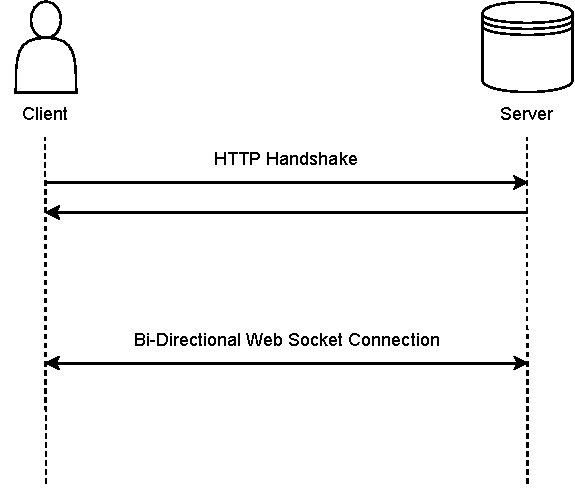
\includegraphics[width=0.5\linewidth]{images/implementation/websocket.pdf}    
    \caption{The WebSocket API provides a bi-directional connection between a client and server, enabling full-duplex communications between the two.}
    \label{fig:websocket}
\end{figure}

A suitable web framework which was ultimately chosen for the project was Django with the Channels extension, which adds support for the WebSockets API. Additionally, with Django offering easy-to-use ORM and templating tools, it was the clear choice for rapid development.

The server sends socket messages through Django Channel’s “Consumer” model, while on the client-side, local JavaScript functions are in charge of receiving, parsing, and sending messages through the socket.


\subsection{Integrating Audio}
After choosing the right web framework, the second most important technology decision was choosing a system to integrate audio into the app, as serving audio in a timely and efficient manner was paramount to the user experience.

The Web Audio API is a relatively new technology, with its release as a W3C recommendation in 2021. It provides a system for loading, processing, and synthesising audio within web applications and offers a high degree of flexibility and modularity. For this project, it was another obvious choice as it is currently the only JavaScript API which supports modular routing, allowing for audio to be manipulated in a number of ways while it is being played.

To do this, audio in the Web Audio API occurs inside of an audio context, where source nodes convey an audio source such as an instrument sample mp3 file. Various audio nodes can then be attached to this source before finally connecting to the context’s destination, for example, the user’s headphones. These audio nodes include gain nodes which allow the volume of the source to be adjusted, and filter nodes which can apply a frequency cutoff to the source, i.e. a low or high-pass filter. Figure \ref{fig:web-audio-api} illustrates a simplified workflow for establishing, manipulating, and outputting an audio source.

By linking frontend controls such as sliders or buttons to functions which modify these audio node properties, users can modify the sound of an audio source as it is being played. Utilising this dynamic node system is crucial for this project to succeed as the requirements specify that users should have control over the sounds as they are being played and/or generated.

\begin{figure}[htb]
    \centering
    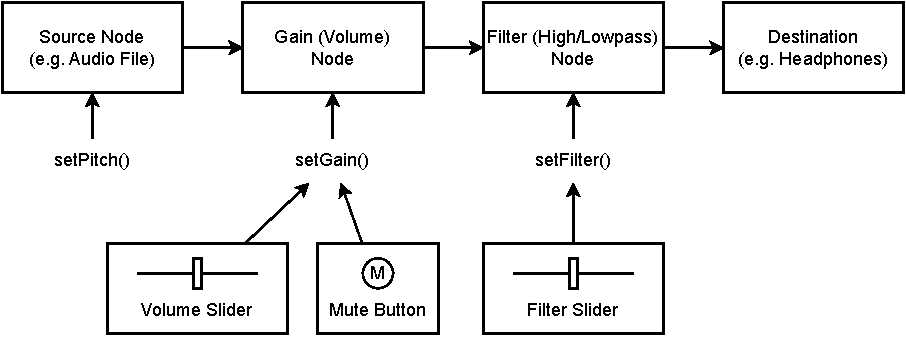
\includegraphics[width=0.7\linewidth]{images/implementation/web-audio-api.pdf}    
    \caption{A simplified audio node diagram, where an audio source is created, then connected to two modifier audio nodes before reaching the context's destination. The setGain() and setFilter() functions are examples of how the interface controls can actively manipulate the sound of a given source (e.g. an instrument sample, ambient sound file, etc.).}
    \label{fig:web-audio-api}
\end{figure}

\subsection{Interface Design}
The interface will be styled using fully custom stylesheets as there is total control over every element of the interface compared to using CSS libraries such as Tailwind or Bootstrap. Although this will increase the implementation time due to styling every element manually, the project’s focus is on creating an engaging and immersive user experience. Decisions which benefit the user experience such as increased control over the site’s appearance are worth the additional time and complexity.

For interactive elements like control surfaces and dynamic visual aspects, local JavaScript scripts will be used alongside jQuery to simplify development.


\section{The Audio System}
The audio system is one of the more novel aspects of this project. Using the Web Audio API to load, manipulate, and deliver sound to the user required many attempts and revisions to get working reliably and consistently. This section will cover some of the technical aspects of creating the musical experience.

\subsection{Tracks and Nodes}
The audio system is comprised of four tracks:
\begin{enumerate}
    \item An ambience track for the ambient mix
    \item A sequencer track for the drum machine
    \item An instrument track for playing the various instruments
    \item A UI track for triggering auditory cues when users interact with controls
\end{enumerate}

Each track is an object which has several audio sources, where each source has a source node, a gain node, and a filter node. Prototype methods are used to manipulate these nodes and UI controls use event listeners to link them to these methods.

For example, the ambience track has seven audio sources which depict the seven ambient sounds users can mix together. Each of these sources has its own gain and filter nodes, allowing each sound to be independently controlled. When a user drags a volume slider, an event listener sees this input and triggers an associated \verb|setGain()| function for whichever sound the slider was associated with. Additionally, this event listener sends a message through the socket so the server can forward the volume update to any other connected users, which then parse this message and update their own gain nodes. See Figure \ref{fig:socket} for an illustration of this example. More information on the socket messages is described later in this chapter.

\begin{figure}[htb]
    \centering
    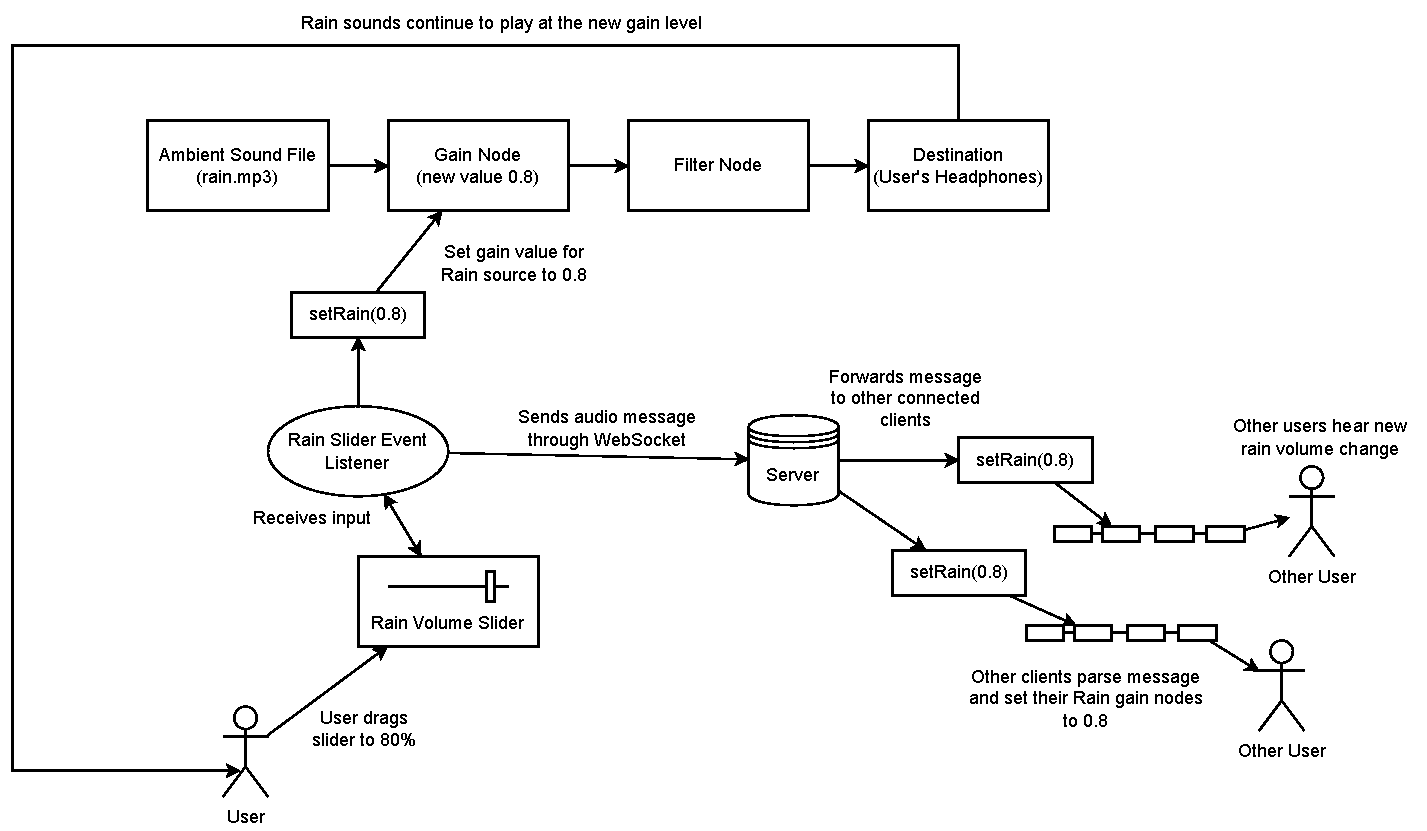
\includegraphics[width=0.8\linewidth]{images/implementation/socket.pdf}    
    \caption{An example of a user interacting with the "Rain" volume slider and how this not only adjusts their own local gain but every other connected user's Rain sample gain as well.}
    \label{fig:socket}
\end{figure}

Each track has its own methods to serve its specific purposes, but all tracks have sources which consist of a similar audio node structure. Instruments, for example, generally have a source node which contains a recording of that instrument playing one note. To create music, however, the instruments need to be able to play lots of different notes.

\subsection{Manipulating Pitch}
To play different notes, a sample is pitch-shifted by either increasing or decreasing its playback speed. All of the instruments apart from the guitar are a single mp3 file of that instrument playing a note at 440Hz, or “A4” in Scientific Pitch Notation (where A is the note and 4 is the octave). By doubling or halving the frequency, the output is the same note in a higher or lower octave. In an octave, there are 12 semitones (i.e. A3 and A4 are 12 notes apart). See Figure \ref{fig:keyboard} for an illustration of this.

\begin{figure}[htb]
    \centering
    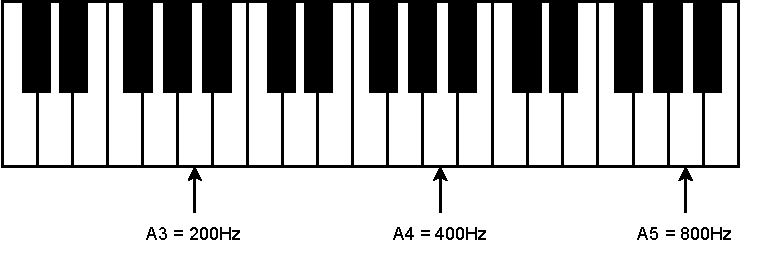
\includegraphics[width=0.7\linewidth]{images/implementation/keyboard.pdf}    
    \caption{A piano keyboard with labels for the A3, A4, and A5 notes.}
    \label{fig:keyboard}
\end{figure}

Audio source nodes in the Web Audio API have a property called “detune”, which offsets the playback frequency by cents. In music, a cent is one-hundredth of a semitone, so setting the detune property to +100 would sound the sample at one semitone higher, and a value of -100 would sound the sample at one semitone lower in pitch. Using this information, a map can be created which maps notes to their corresponding detune value. For example, A4 would be +0, B4 would be +200, F4 would map to -400, etc.

The JavaScript code in Listing \ref{lst:notes} creates a map between notes in Scientific Pitch Notation to the detune value in cents required to pitch a sample playing at 440Hz to that note.

\begin{lstlisting}[float, caption={Creates a map "noteCentsOffsets" between notes in Scientific Pitch Notation to the detune value in cents required to pitch a sample playing at 440Hz to that note}, label=lst:notes]

    // Generate equal temperament notes list
    const range = (start, stop) => Array(stop - start + 1).fill().map((_, i) => start + i);
    const octaveRange = range(0, 8).map(val => [val, val - 4]);
    const semitoneOffsets = [
        ["C", -9], ["C#", -8], ["Db", -8], ["D", -7], ["D#", -6], ["Eb", -6], ["E", -5], ["F", -4],
        ["F#", -3], ["Gb", -3], ["G", -2], ["G#", -1], ["Ab", -1], ["A", 0], ["A#", 1], ["Bb", 1], ["B", 2],
    ];
    const notes = octaveRange.reduce((ob, [range, multiplier]) => semitoneOffsets.reduce((ob, [note, semitones]) => ({
        ...ob,
        [note + range]: 440 * Math.pow(2, (semitones + (multiplier * 12)) / 12),
    }), ob), {});
    
    
    // Map each note to its offset in cents (100 cents p/ semitone) relative to 440 Hz
    const noteCentsOffsets = {};
    Object.keys(notes).forEach(note => {
      const frequency = notes[note];
      const centsOffset = 1200 * Math.log2(frequency / 440);
      noteCentsOffsets[note] = centsOffset;
    });

\end{lstlisting}

After this, the instrument’s \verb|sound()| method can take in a note parameter, and then offset the source node of the specified sample by looking up the note in the offsets mapping. For example, \verb|instrumentTrack.sound(“piano”, “C6”)| would create a new source using the \verb|piano.mp3| file, detune it by +1500 cents, and then play it. This is how instruments can play different notes with only one audio sample, and by creating pitches this way, fewer audio files are required to be loaded by clients, lowering the network requirement for users to use the app and therefore increasing its accessibility.

\subsection{Harmonising Instruments}
In music, two notes can sound generally either sound “consonant/harmonious” or “dissonant”, where the former typically sounds more pleasing. Notes can sound dissonant when the ratio between their respective frequencies is farther from being an integer. For example, the notes C and G sound consonant because their frequency ratio is 3:2, while the notes F and B have a frequency ratio of 64:45, and subsequently these notes sound dissonant and generally unpleasing when played together.

In this project, instruments are limited to playing notes in the G flat major pentatonic scale. The pentatonic scale is unique because all of the notes in the scale sound consonant with all the other notes, meaning no matter what combination is playing, there will not be any unpleasing dissonance. This means that the instruments will never clash harmonically and can be programmed to play (essentially) random notes so long as they are in the correct scale.

Harmony, however, is not the only aspect of creating music which is perceived as cohesive and/or natural. The instruments need to play in complementary styles and in a way which sounds organic.

\subsection{Generating Organic-Sounding Music}
Each instrument follows a set of pre-defined rules which were set to make them sound natural and human-like. The most comprehensive example is the piano part, which this section will describe.

First, a random number is generated with a minimum value of zero, and a maximum value of 6-26, which is set by the user using the “density” slider. Then, a switch statement will attempt to match that number to a pre-defined variation.

\begin{itemize}
    \item If the number is 0, the piano generates a chord comprised of three notes
    \item If 1, the piano plays a smaller chord comprised of two notes
    \item If 2 or 3, a single note is played
    \item If 4, the piano plays two notes in succession
    \item If 5, a triplet is played (three notes in succession)
\end{itemize}

If the number does not match any of the cases, then the piano will play nothing. A new number is generated every half-beat, which means eight numbers will be generated and matched to a variation through the course of one bar of music.

When compared to a more rudimentary method of generating melodies, for example by choosing a random note every beat and then playing it, these rules generate a piano part which sounds more organic and musically purposeful. Figure \ref{fig:piano} compares the notation of an excerpt of the piano’s algorithm with a high density with one that generates a random note for every beat.

\begin{figure}[htb] 
    \centering
    \begin{subfigure}[b]{0.45\textwidth}
        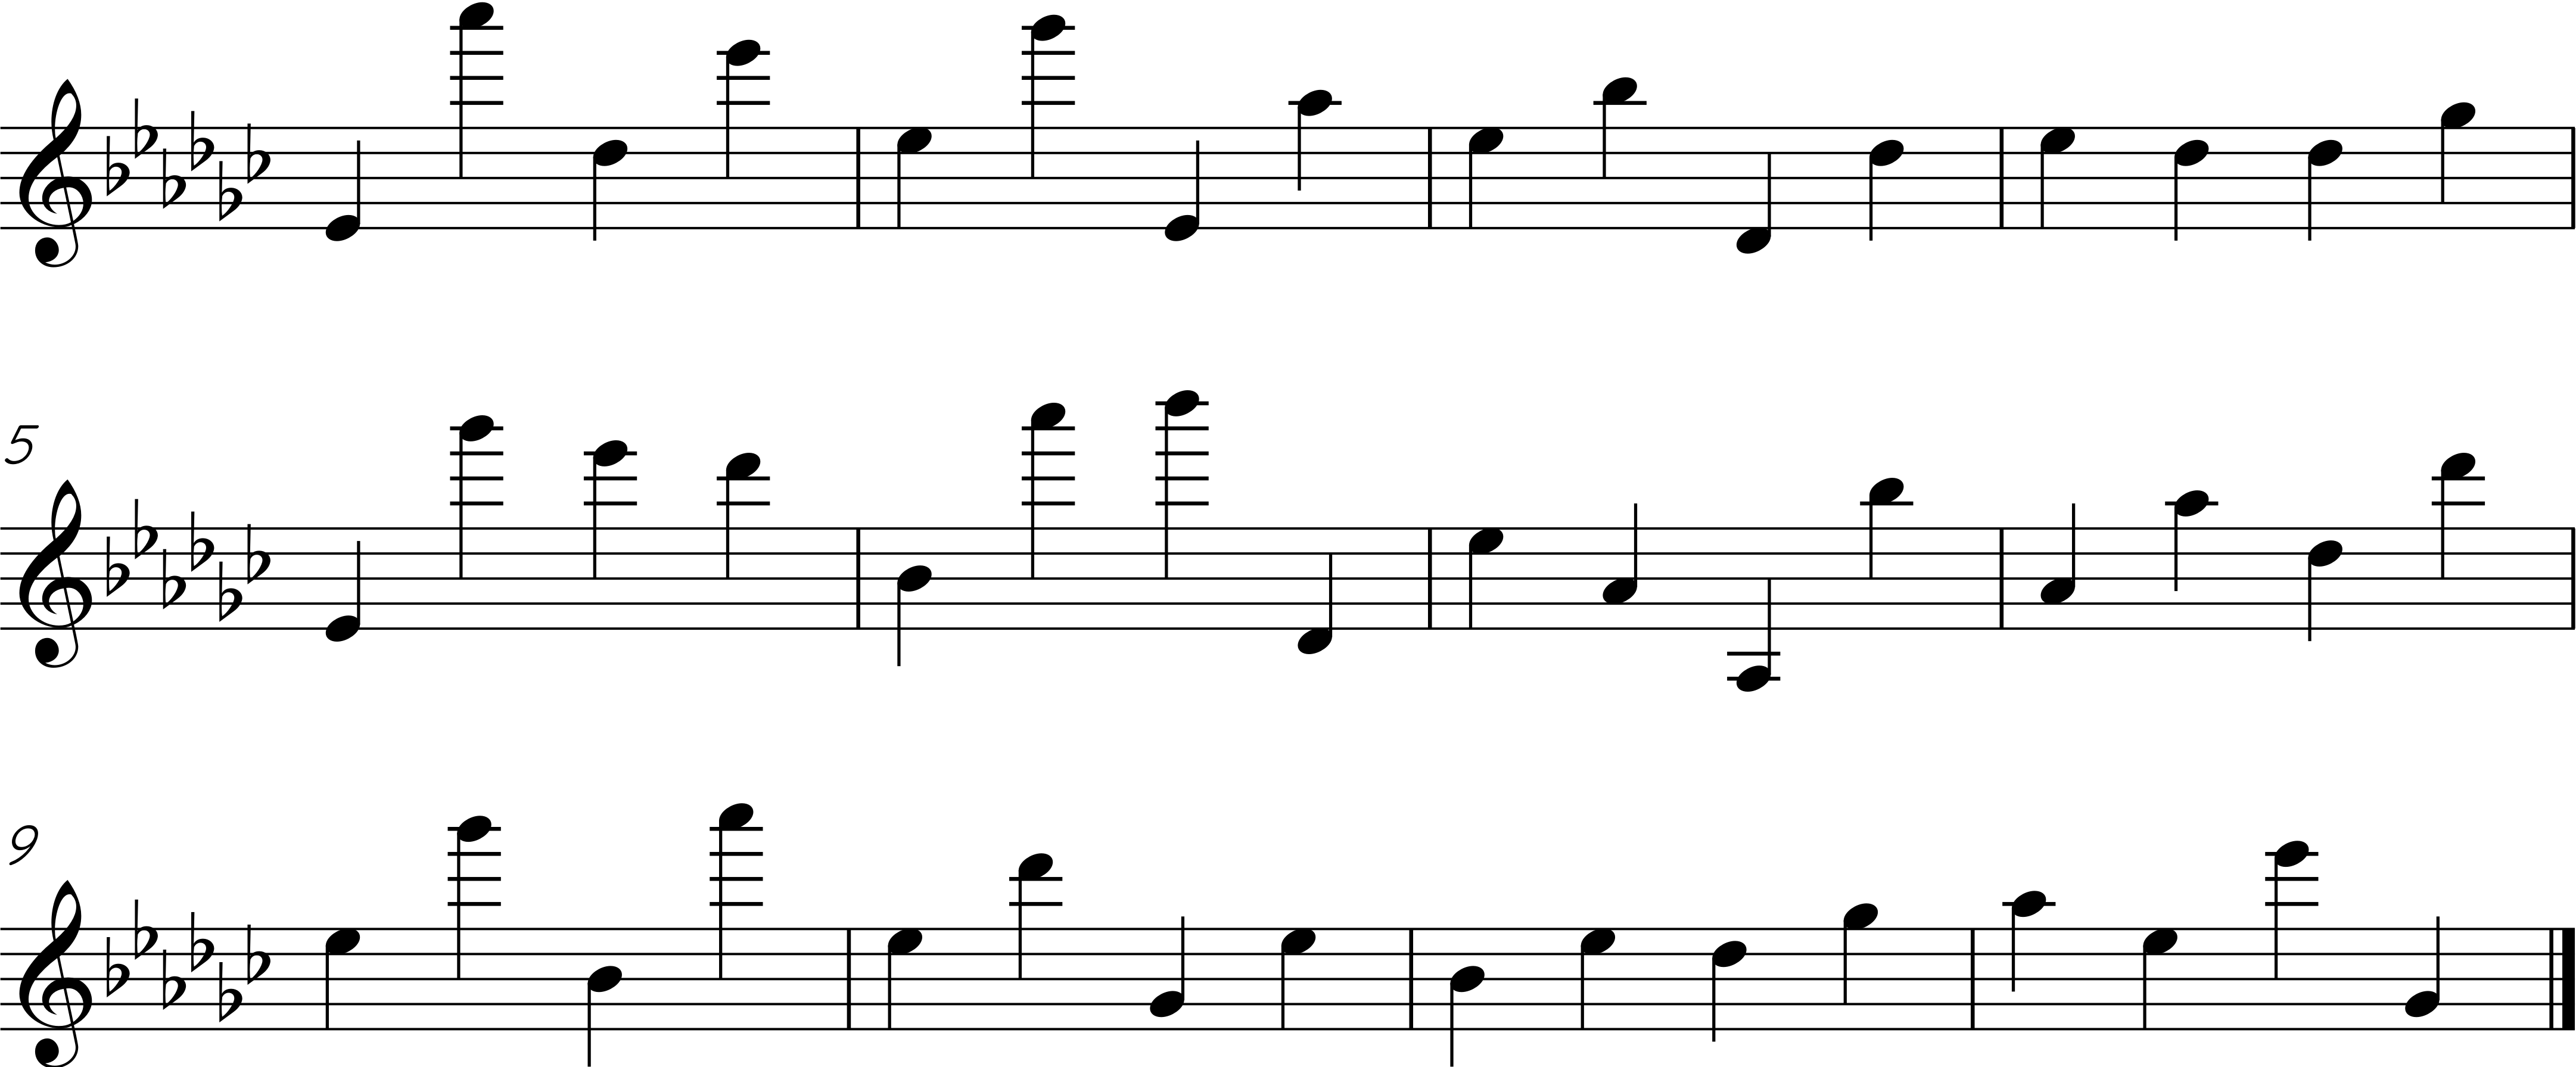
\includegraphics[width=\textwidth]{images/implementation/generated-piano-basic.png}
        \caption{A basic algorithm for generating a melody by choosing a random note of the scale every beat.}
        \label{fig:generated-piano-basic}
    \end{subfigure}
    ~
    \begin{subfigure}[b]{0.45\textwidth}
        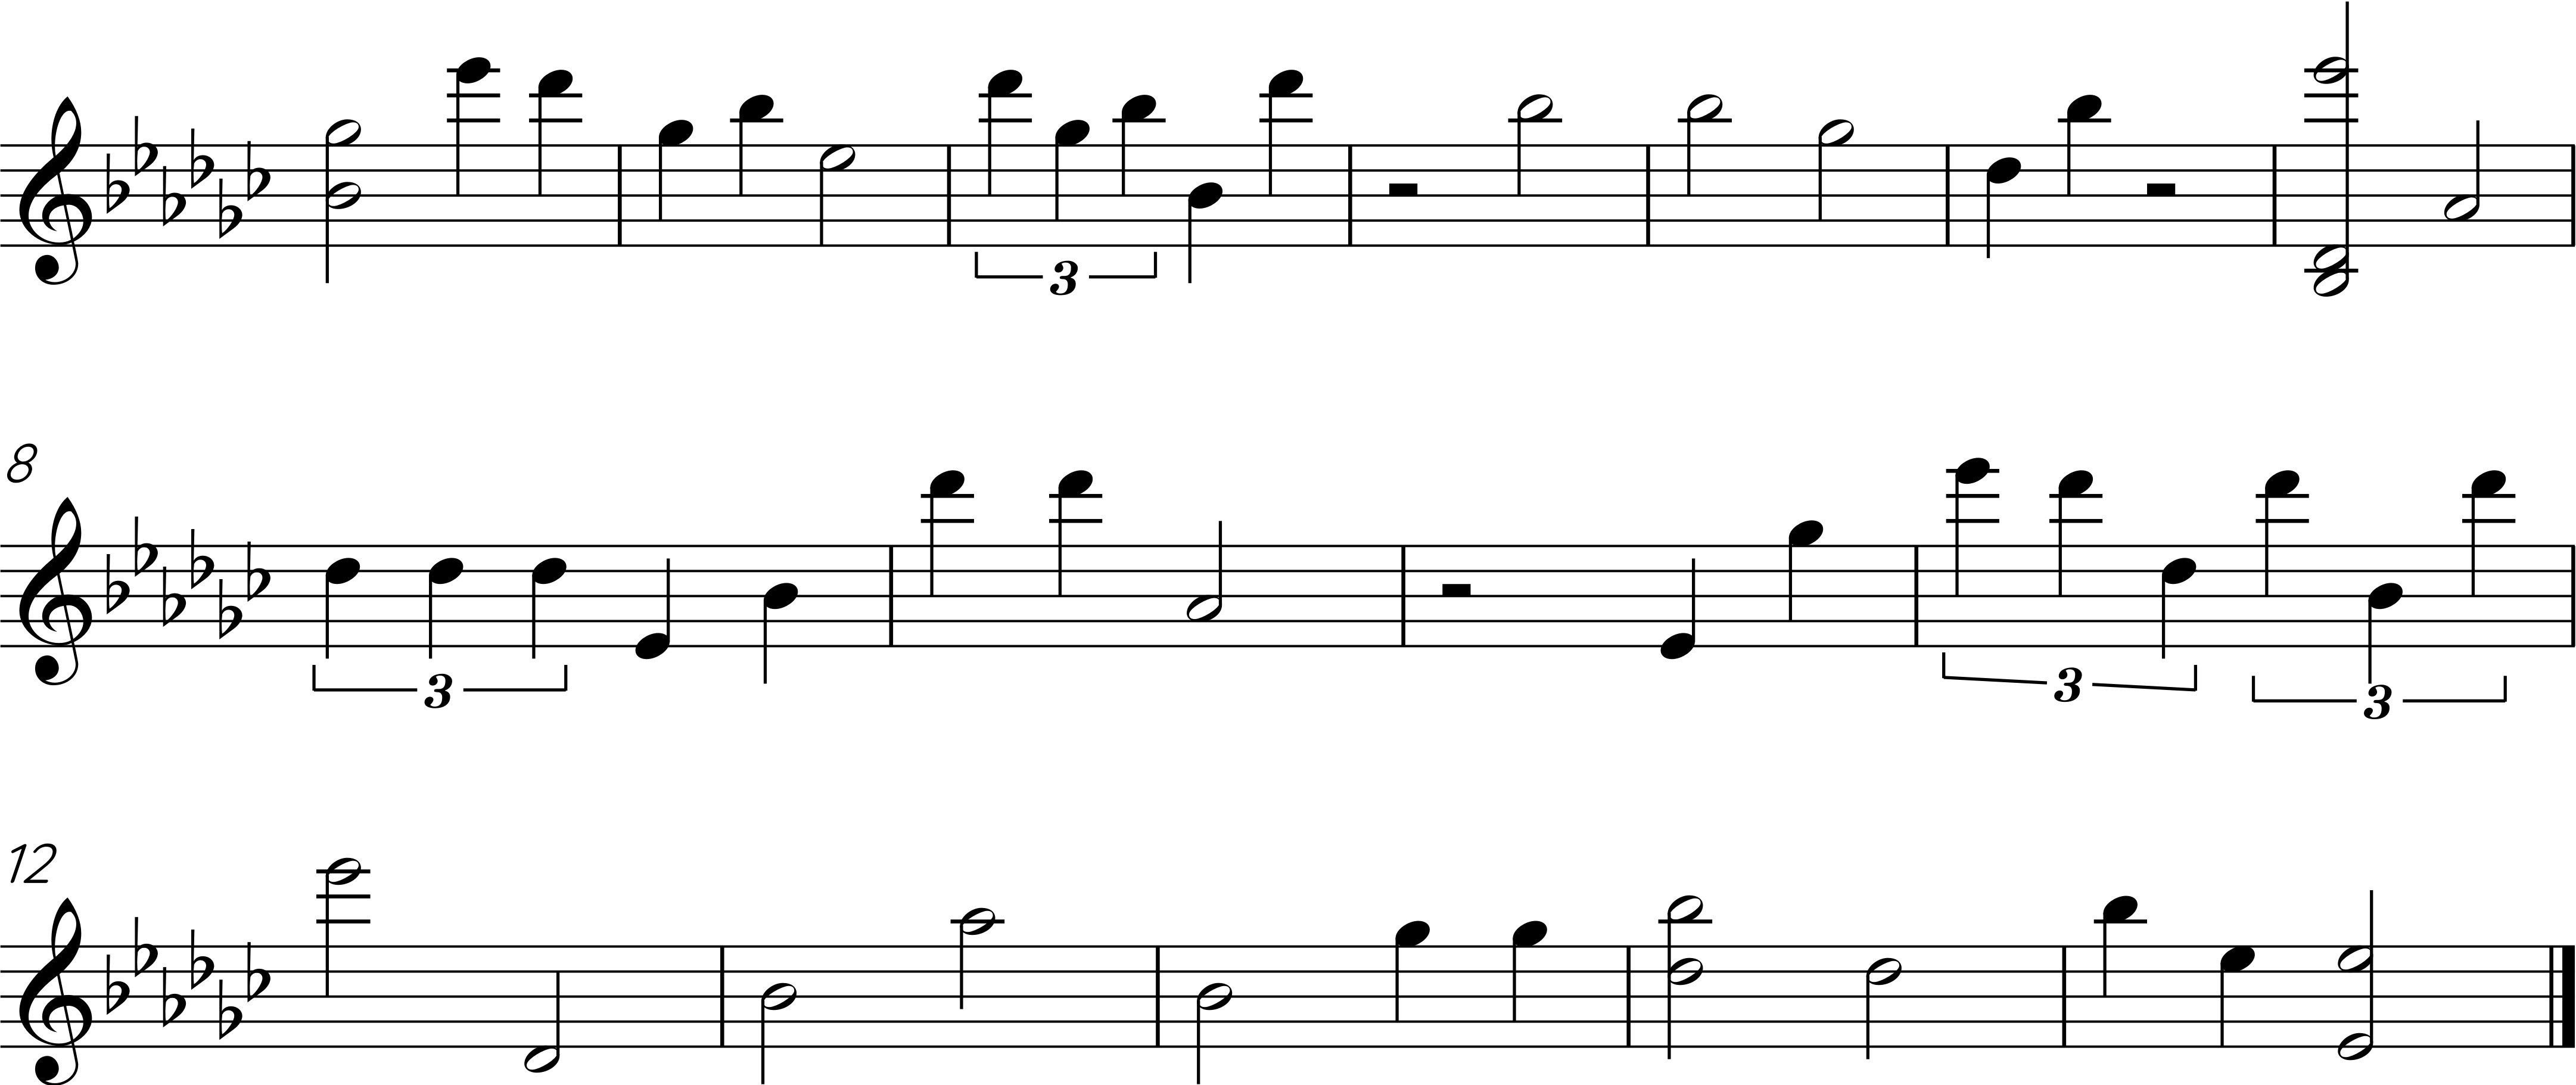
\includegraphics[width=\textwidth]{images/implementation/generated-piano.png}
        \caption{Using the system's algorithm to generate a piano part based on a number of simple cases.}
        \label{fig:generated-piano}
    \end{subfigure}
    ~
    \caption{
    Compared to the \subref{fig:generated-piano-basic} basic algorithm, the \subref{fig:generated-piano} proprietary algorithm creates a much more natural and realistic piano part.
    }\label{fig:piano}
\end{figure}

\subsection{Creating Reactive Instruments}
Not only do the instruments need to sound natural, but their generation should be able to be manipulated by the user. In the piano part, there is a density slider which the user can adjust. By increasing the density, the number which gets inputted into the piano algorithm decreases. This means that there is a higher probability for one of the cases in the switch statement to match, and therefore, a lower probability for the piano not to play at a given timestep. This results in a denser melodic line. This is similar to the marimba instrument’s implementation, where the density decreases the probability of it not playing at a given timestep, and sliding the density to the maximum value leaves the marimba consistently playing a note four times per beat.

The electric guitar instrument, however, has a completely different behaviour from the rest of the instruments in the system. Instead of picking a note or notes to play at a given timestep, the guitar is pre-programmed with a concrete set of MIDI recordings lasting two bars of music each, where each phrase has an associated “intensity” and “density” label. For example, if the user sets the intensity to “medium” and the density to “sparse”, the guitar will randomly pick a pre-recorded phrase which is labelled with medium intensity and sparse density, playing that sample at the start of the next two measures.

The guitar is defined this way to allow for greater expressive control over the instrument, allowing pitch bends, vibrato, and more complex rhythmic phrasing to be included in the samples, which would not be possible if the guitar used the same system as the other instruments.

A downside to this method of implementing the guitar part is that when a user changes a modifier, it will only start playing in the updated parameters after the current two-bar sample finishes playing. This means there is a delay between the user changing the slider and the guitar responding to that change, however, the benefits of greater expressive control were worth this compromise since the rest of the instruments did react immediately to the user’s changes.

Many of the instruments have a “Filter” slider which adjusts the instrument’s filter node, adding either a low or high-pass filter to the instrument. This works by cutting off the frequencies either below or above (depending on the type of filter) a target frequency. By sliding a filter slider to the left, a low-pass filter begins to cut frequencies higher than the slider’s value. Similarly, sliding to the right cuts off frequencies below the target. It is also worth noting that the relationship between pitches and frequencies follows a logarithmic scale, so the linear positions of the filter sliders have to be converted to that scale so that when a user drags the slider linearly, the apparent filter cutoff follows a roughly audibly linear scale.

Adding filters to the instruments can drastically change their tone, with a low-pass filter “muffling” the sound, and a high-pass creating a “tinny” sound when pushed to their respective extents. It was worth adding these so that the user has even more control over the tone of the instruments.

\section{Synchronising with Sockets}
One of the most challenging aspects of this project was ensuring the musical experience was identical across all connected users. This was done by sending and receiving messages through the WebSocket connection. When a user changes a control or modifier in the app, a message is sent to the server indicating which control was changed alongside its updated value. The server forwards all socket messages to any other connected user alongside sending a regular pulse which acts as the music beat.
By making sure every change to the app is sent through to the users in an audio room, the system can ensure consistency across those connected users. This came with additional complexities which had to be resolved for the app to work efficiently and consistently. This section describes some of the technical factors behind creating the finished product.

\subsection{Message Format}
The messages sent through the socket follow a specific format which was developed to efficiently convey system control and state updates. Any message that involves audio includes \verb|‘type: ‘audio_message’| at the beginning of the message to indicate that the app should then parse the rest of the message.

These messages typically contained a \verb|track| field, which indicated which track the change was for. For example, when a user mutes a sequencer sample, the track field would be \verb|'sequencer'|, or if the user drags an ambience volume slider, the track field would be \verb|'ambience'|. To parse audio messages, switch statements are used to determine what category of control was made. For each track type, there were subsequent fields such as \verb|'target'|, \verb|'instrument'| or \verb|'sliderID'|.

Audio messages contain a \verb|'user'| field, which was implemented during testing as when a client sent audio messages to the server, the server would forward that message to all connected users, including the client who sent the message. A result of this was “rubber-banding”, where after making a change to the app, there would be a brief delay before that change was then echoed back to the client and that state update would repeat itself. This was not noticeable with changes such as toggling a track on or off, but when sliding a control slider, the slider would flicker back and forth as it received the client’s own commands while the user was still dragging the slider, typically after <100ms. Fixing this involved sending the username as a field within the socket message. Then, clients could ignore any messages that had their username attached, removing the rubber-banding effect completely.

Instruments, alongside what notes they play, are also triggered by socket messages. Every beat, the server sends messages about the notes that each instrument should play. These can be randomly generated, but since they are generated server-side and then sent to the clients, the random notes are the same notes for each connected user, ensuring a consistent experience.

\subsection{Sending Beats Consistently}
The notes are not the only thing that is required to be consistent, as the rhythm of the music needs to be strictly in time with imperceivable fluctuations in beat consistency. To synchronise the sequencer beats and instrument cues, the server sends beat messages every second, which means the system runs at 60 bpm. This can be thought of as a form of metronome for the clients to play in time with.

At first, the server attempted to send a pulse every 200ms, which at the time was how long each of the 16 sequencer timesteps was supposed to last. This was done by creating an asynchronous server-side worker which sent out the sequencer beat message alongside any instrument cues which would occur on that timestep, then slept for 200ms. When running the server locally this worked fairly consistently, however, once deployed, the latency was very inconsistent and beats would regularly arrive late.

After experimenting with different sleep durations, it was apparent that regardless of the sleep duration, there was ~200ms additional latency which when built up over the 16 timesteps added up to over 3 seconds of average unintended delay. Additionally, the total duration of a bar of music would last anywhere between 5100 and 6600ms. This was obvious when using the sequencer, as beats would drastically slow down and speed up over time.

To fix this, the server should no longer rely on sleeping after sending socket messages, and it was apparent that the time taken to send those socket messages would vary by a large margin. The solution was to reduce the amount of socket messages by over 80\% and instead send one pulse every 1000ms rather than every 200ms. This pulse would also not depend on how long the previous task took but instead use the server’s very accurate system time to measure the time until the next system second, then delay by that amount.

By doing this, the average bar duration variance fell from over 1500ms to <25ms, an approximately 98\% reduction. This led to an audible improvement in beat consistency, as beats would arrive with imperceptibly small fluctuations, with most of these due to the internet connection with the remote server, which is located in London.

Reducing the server’s update frequency from 4 updates per beat to 1 resulted in a major refactoring to the socket format, particularly to the sequencer. Previously, the server would send 16 updates per bar which directly triggered the sequencer to play one of its timesteps. After the change, clients receive one server beat update every four sequencer timesteps. Because of this, when a server beat message is received by the client (every 1000ms), it plays the first of the timestep of the beat instantly, then sets three internal timeouts: 250, 500, and 750ms respectively, where each of these timeouts plays one of the other subsequent sequencer timesteps. For example, when the client receives “Beat 1”, the sequencer plays timestep 0, waits 250ms, plays timestep 1, waits, plays 2, waits, and plays 3. Then in 250ms time, the client should expect to receive “Beat 2” from the socket which triggers sequencer timesteps 4-7.

By combining occasional but accurate server pulses with local timeouts, the user experiences a very consistent rhythm which is important for the immersive aspect of the app.
